% Auto-generated editable source. Edit freely in VS Code.
% Parallel source; the live site is pages/proj-latent-coordinates.html.
\documentclass[11pt]{article}
\usepackage[margin=1in]{geometry}
\usepackage{graphicx}
\usepackage{hyperref}
\usepackage{booktabs}
\usepackage{xcolor}
\definecolor{aidred}{HTML}{A8324A}
\definecolor{aidpink}{HTML}{CF4D87}
\hypersetup{colorlinks=true,linkcolor=aidpink,urlcolor=aidpink,citecolor=aidpink}
\newcommand{\finding}[2]{\par\medskip\noindent{\color{aidred}\textbf{Finding #1.}}~#2\par\medskip}

\title{Which Latent Coordinates Drive World-Model Dynamics?}
\author{Saanvi S. Subramanian \\ \small California Institute of Technology}
\date{\small poster, Robotics World Modeling @ NeurIPS 2026 \quad\textbullet\quad sole author}
\begin{document}
\maketitle

\begin{abstract}
\noindent A world model predicts what it will observe next, and to do that it holds an internal state. People read variables out of that state with a probe and treat a readable variable as one the model uses. Those are different properties. I build a label-free test that uses only actions and the frozen model's own next-observation predictions: a candidate coordinate is a plane in the latent space, and the test asks whether rotating the state inside that plane reproduces the effect of an extra action. A coordinate that passes is one the dynamics use; a coordinate that is only decodable can fail. Across three two-joint arms that differ only in how the image depends on the joints, the coordinates a model builds follow what the observation makes separable, not the number of actuators.
\end{abstract}

\section*{Decoding is not use}
The criterion discovers coordinates from actions and the frozen model's own predictions alone, with no pose labels, supervised decoder, or other ground truth entering before scoring. A candidate coordinate is a plane in latent space. The test rotates the state inside that plane and asks whether the rotation imitates an extra action, judged by the model's next-observation predictions. A coordinate the dynamics use passes; a coordinate that is only decodable can fail.

The two questions give different answers. In the parent project's shuffled-action control, heading decodes to within 20 to 24 degrees, but the conjugate plane sits 69 to 83 degrees away. The variable is present, held in a decaying trace of the last visible observation, and the dynamics do not act on it.

\begin{figure}[h]\centering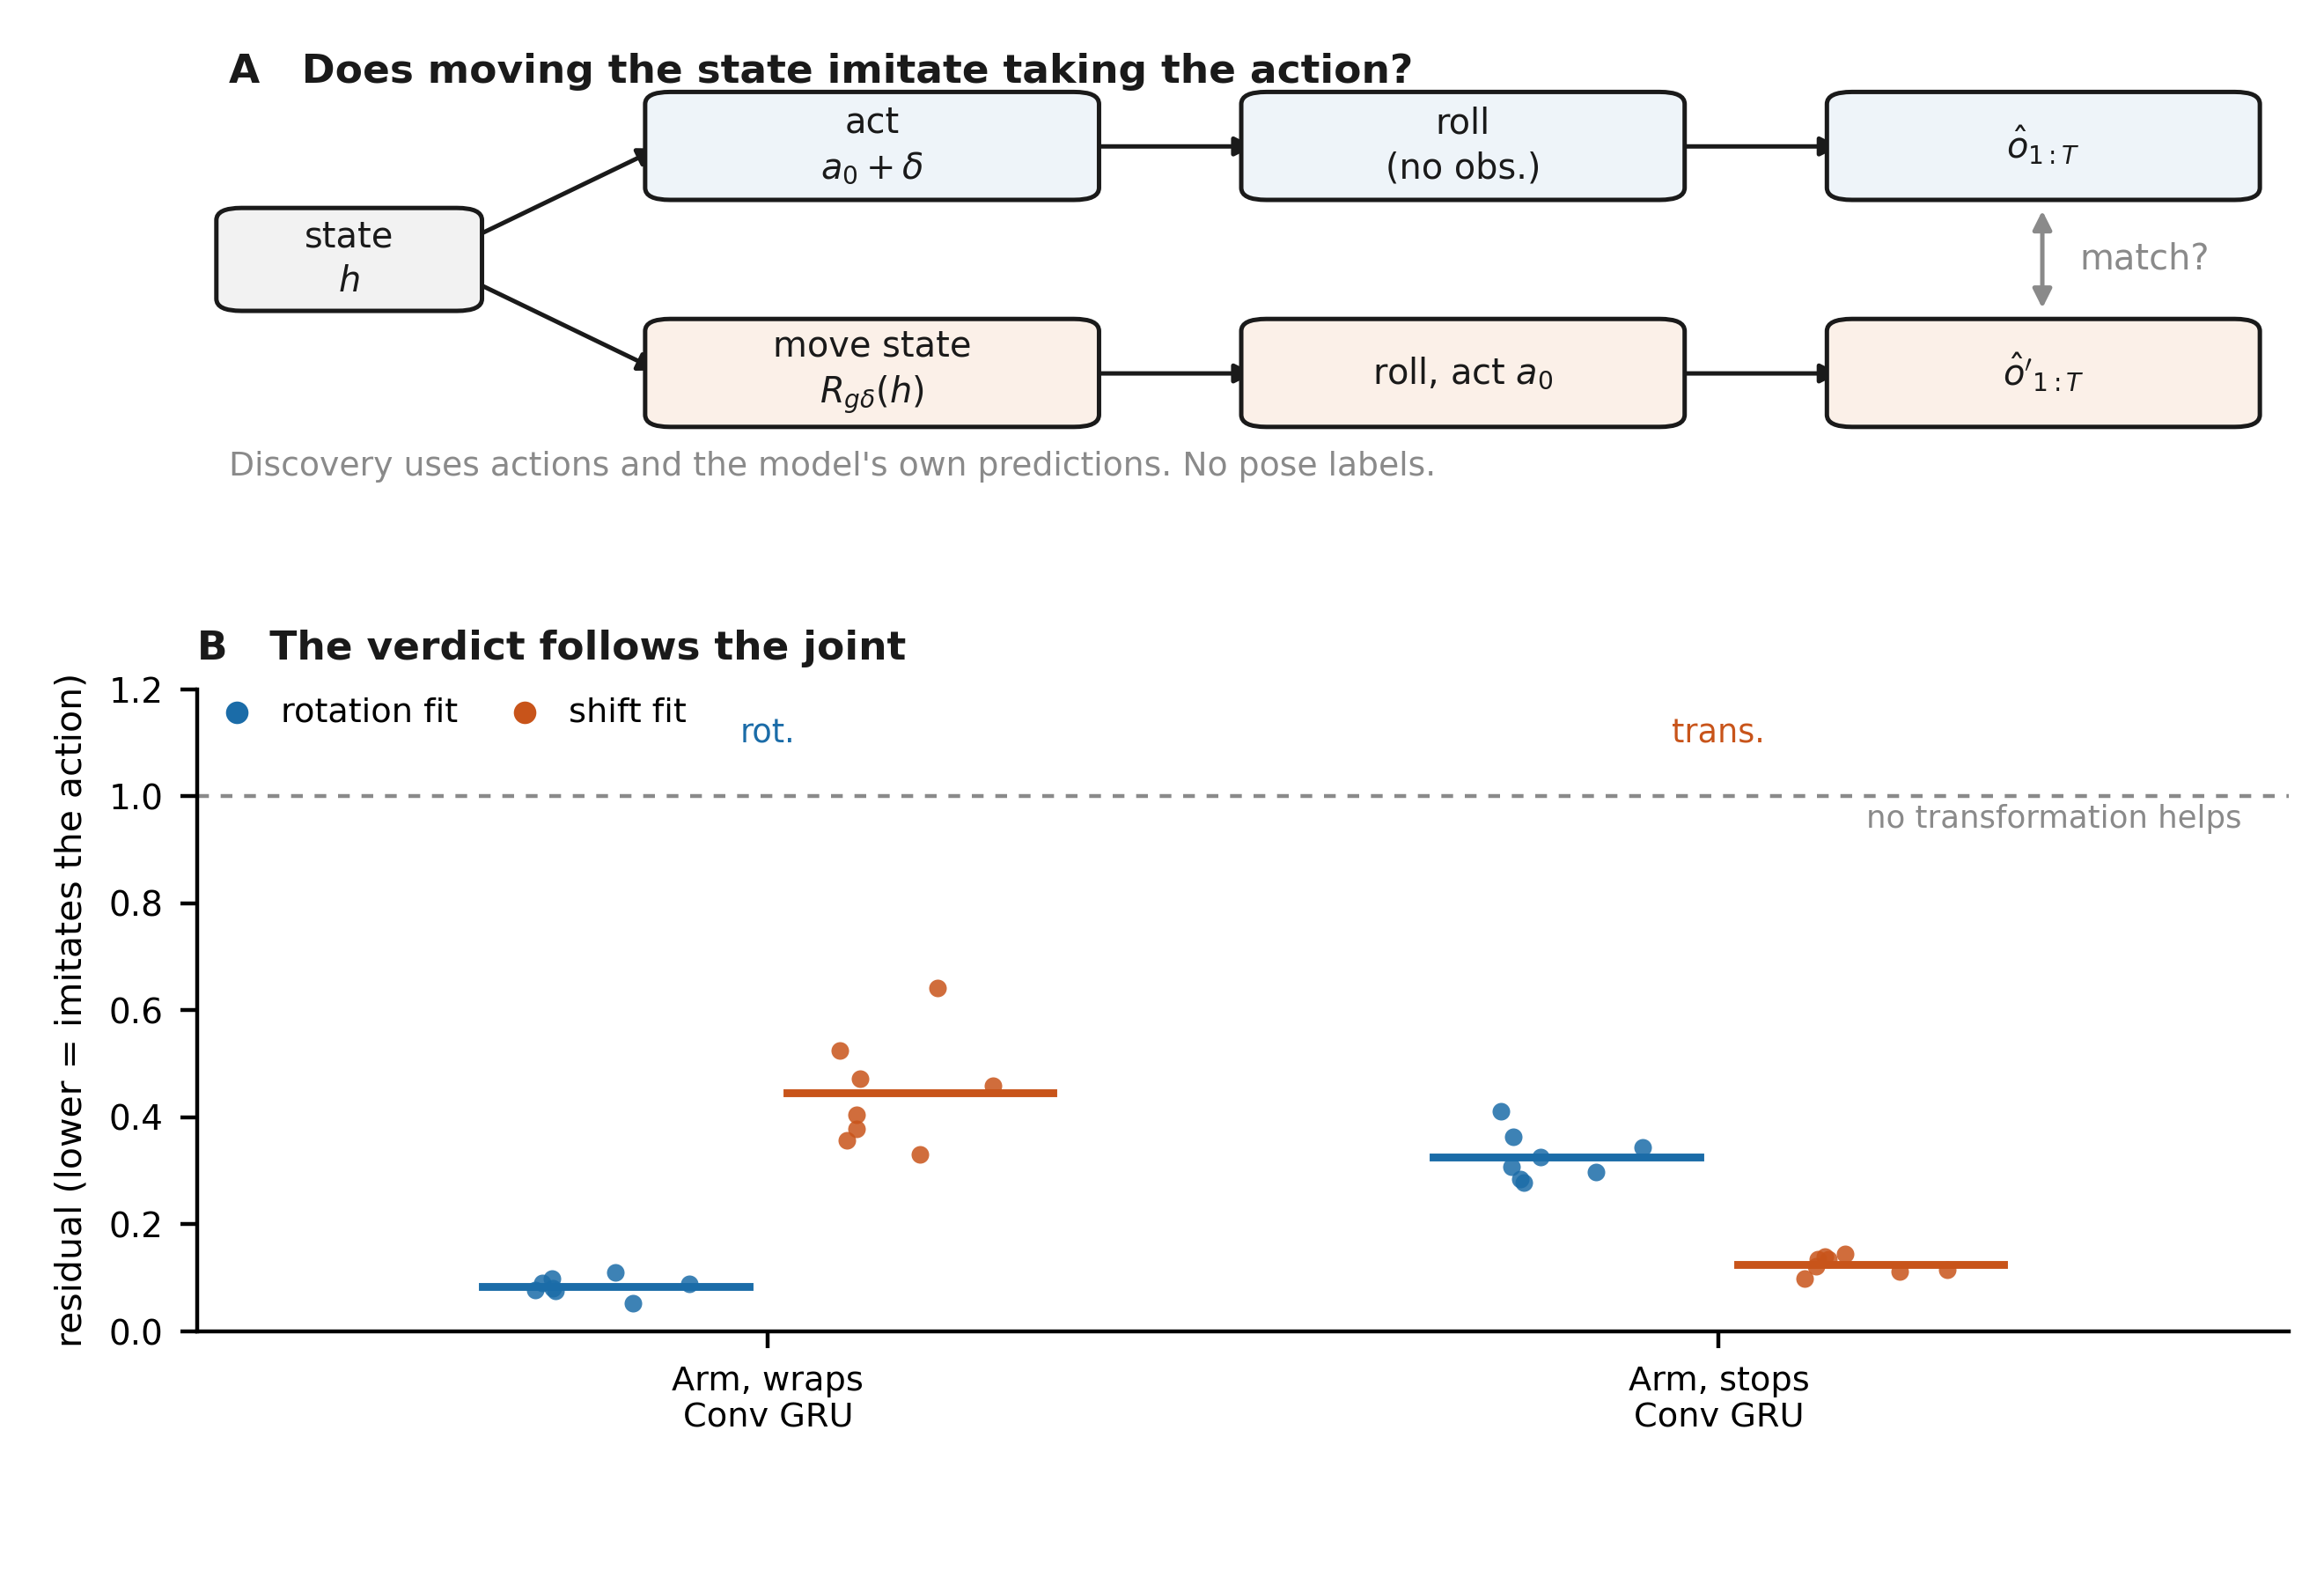
\includegraphics[width=\textwidth]{../../assets/images/projects/latent/criterion.png}
\caption*{\textcolor{aidred}{\textbf{Figure 1. The criterion separates decoding from use.}} A candidate coordinate is a plane in latent space; rotating the state inside it is scored by how well it reproduces an action in the model's own next-observation predictions, against a variance-matched null. A coordinate the dynamics use clears the null, while one that is only decodable does not.}\end{figure}

\finding{1}{Decoding and use come apart. A probe can read a coordinate out of a world model's latent state while the dynamics do not treat it as a coordinate, and the gap is measurable: in the shuffled-action control, heading decodes to 20 to 24 degrees while the plane the dynamics use sits 69 to 83 degrees away.}

\section*{The observation decides which coordinates get built}
I trained the same model on three two-joint arms that differ only in how the image depends on the joints, with dynamics, action space, image size, sensor noise, architecture, training budget, and the estimator held fixed. The coordinate the model builds follows what the image makes separable.

\begin{center}
\begin{tabular}{lll}
\toprule
environment & what the image depends on & coordinates built \\
\midrule
serial arm & q1 and q1+q2, proximal dominant & one, at (1,0) \\
parity arm & q1+q2 only & one, at (1,1) \\
decoupled arm & q1 and q2 separately & two, at (1,0) and (0,1) \\
\bottomrule
\end{tabular}
\end{center}

\finding{2}{Which coordinates a model builds is set by the observation, not the actuators. The coordinate tracks what the image makes separable: a serial arm gives one coordinate, a parity arm one, and a decoupled arm two. Both joint angles decode in every case, but the proximal joint's conjugacy margin is six times the distal joint's, so extra actuators do not buy extra coordinates. A serial chain cannot be made distal-dominant, which is a fact about kinematics, not about learning.}

\section*{Limitations}
Established in this setting: the dissociation between decoding and use, and the dependence of which coordinates appear on observation separability. Not established, and not written as if it were: anything beyond 16x32 synthetic RGB, small convolutional GRUs, and two degrees of freedom; anything about non-circular coordinates, since the criterion as implemented tests a planar rotation, one group action among many; any comparison with the probing, disentanglement, or activation-patching literature, so ``probes overstate what is used'' stays a hypothesis until those baselines are run; and anything about real robots or real video.

\end{document}
